\documentclass[a4paper,11pt]{article}

% caricamento dei pacchetti

\usepackage[T1]{fontenc} % codifica dei font
\usepackage[utf8]{inputenc} % lettere accentate da tastiera
\usepackage[italian]{babel} % lingua del documento

\usepackage{lipsum} % genera testo fittizio

\usepackage{url} % per scrivere gli indirizzi Internet

\usepackage{booktabs} % per tabelle: permette di usare \toprule etc

\usepackage[colorlinks]{hyperref} % per aggiungere link al testo

\usepackage{graphicx} % per includere immagini
\usepackage{wrapfig} % per immergere le immagini nel testo

\begin{document}

% Creazione del titolo
\title{Introduciamo \LaTeX\  al Peano}
\author{Andrea Mezzalira}
\renewcommand{\today}{23 Ottobre 2017}

\maketitle

% creazione del sommario (abstract)
\begin{abstract}
    \lipsum[1]
\end{abstract}

% Creazione dell'indice
\tableofcontents

% Inizio del documento

\section{Plain Text}
Scrivete il vostro documento come volete, potete
fare delle righe lunghe o corte, sarà poi \LaTeX\  a sistemarle
per bene!

Le righe vuote terminano i paragrafi.


\section{Displayed Text}
Usate l'ambiente ``quote'' e ``quotation'' per aumentare il rientro del testo, utilissimo per evidenziare o citare del testo:

\begin{quotation}
Bla bla bla!

\em Ed ecco del testo in italic

\end{quotation}





\section{Liste}

\begin{enumerate}
\item 
L'ambiente ``enumerate'' crea delle liste numerate.
\end{enumerate}


Gli {\em item} in una lista possono contenere diversi paragrafi 

\begin{itemize}
  \item L'ambiente ``itemize'' crea liste con i  ``bullets'' come questo.
\end{itemize}

\noindent Infine, l'ambiente ``description'' vi permette di personalizzare le liste
\begin{description}
    \item[A] ad esempio con una lettera.
    \item[oppure con qualcosa di pi\'u lungo] in questo modo
\end{description}

\section{Tabelle}


Ecco una semplice tabella, inserita in un ambiente centrato per evidenziarla meglio

\begin{center}
Numbers of Computers on Earth Sciences Network, By Type.

\begin{tabular}{lr}
Macintosh   &   175 \\
DOS/Windows PC  &   60  \\
Unix Workstation or server  &   110 \\
\end{tabular}
\end{center}



Un altro esempio più pulito: la tabella
\begin{center}
\begin{tabular}{ll}
\toprule
Alcaloide & Origine \\
\midrule
atropina  & belladonna \\
morfina   & papavero \\
nicotina  & tabacco \\
\bottomrule
\end{tabular}
\end{center}
mostra l’origine di tre alcaloidi.


Di seguito invece una tabella più complessa, con i contorni:
\begin{center}
\begin{tabular}{|l|c|p{3.5in}|}
\hline
\multicolumn{3}{|c|}{Places to Go Backpacking}\\ \hline
Name&Driving Time&Notes\\
&(hours)&\\ 
\hline
Big Basin&1.5&Very nice overnight to Berry Creek Falls from
either Headquarters or ocean side.\\ 
\hline
Sunol&1&Technicolor green in the spring. Watch out for the cows.\\ \hline
Henry Coe&1.5&Large wilderness nearby suitable for multi-day treks.\\ \hline
\end{tabular}
\end{center}

Notate la differenza tra \verb!\midrule! e \verb!\hline!.




\section{Formule ed equazioni}

Formule semplici come $x^y$ or $x_n = \sqrt{a + b}$ possono essere scritte direttamente lungo il testo inserendo la formula tra dollari.

Se volete utilizzare il simbolo dollaro ad esempio in questo modo \$2000,
dovete utilizzare il comando \verb+\$+.
\\

Per equazioni più complicate potete utilizzare l'ambiente  ``equation'' 
\begin{equation}
\label{prima_equazione}
\left[
{\bf X} + {\rm a} \ \geq\ 
\underline{\hat a} \sum_i^N \lim_{x \rightarrow k} \delta C
\right]
\end{equation}
ma ci sono moltissime alternative!

\dots quando Einstein propose l’equazione
\begin{equation}
\label{eqEinstein}
E = mc^2
\end{equation}
uno spasso!

Potete anche rendere l'equazione non numerata
\begin{equation}
    \lim_{x\to 0} \frac{\sin x}{x}=1 \qquad 
    \lim_{n\to +\infty}f_n=\delta
\nonumber % ecco come togliere il numero. Ma ci sono alternative 
\end{equation}

Notate che potete sempre richiamare l'equazione \ref{prima_equazione} 
nel testo usando \verb!\label! e \verb!\ref!. 


\section{Immagini}

Anche qui ci sono varie opzioni. Utilizzeremo qui il pacchetto \verb!graphicx!
Si possono modifica l'altezza, la larghezza, la scala, la posizione\dots

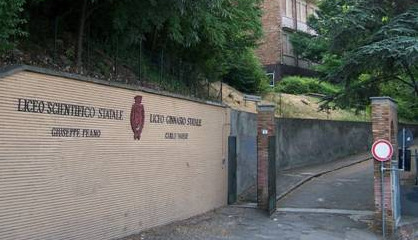
\includegraphics[scale=.5]{peano.jpeg}

Talvolta si potrebbe voler avvolgere una figura con il testo.
E' possibile farlo utilizzando il pacchetto \verb!wrapfig!.

\begin{wrapfloat}{figure}{I}{0pt}
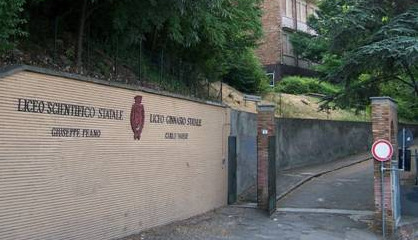
\includegraphics[width=0.5\textwidth]{peano.jpeg}
\end{wrapfloat}
Per avere un buon risultato, possono servire
alcuni aggiustamenti manuali.

\lipsum[1]


% Bibliografia
\begin{thebibliography}{9}
\bibitem{pantieri:arte}
Pantieri, Lorenzo e Tommaso Gordini (2017),
\emph{L’arte di scrivere con \LaTeX},
\url{http://www.lorenzopantieri.net/LaTeX_files/ArteLaTeX.pdf}.
\end{thebibliography}

\end{document}

